\part*{Lecture 4: Treasury Futures, the Basis Trade, and Swaps}
\addcontentsline{toc}{part}{Lecture 4: Treasury Futures, the Basis Trade, and Swaps}
\beginlecture{04}

Week~4 is the final class session of FINM~37400 (Week~5 is the project and the
closed-book exam; no class meeting). The single 144-minute session covers
three notebooks and revisits a fourth: Treasury futures (\emph{4.2}), with
the cheapest-to-deliver (CTD), conversion factors, gross/net basis, implied
repo, and the embedded options the short holds; swaps (\emph{5.1}), from the
size of the market through the swap-rate formula and the puzzle of negative
swap spreads; a cameo review of floating-rate notes (\emph{2.4}) against
\emph{4.1 Forward Pricing}, which was assigned as reading rather than
lectured on; and a one-sentence preview of the \emph{5.2 Swap-Spread Trade}
case that anchors the next lecture.

\begin{tipblock}
\textbf{Audio dropout.} The lecture recording lost microphone input from
about 28:10 through 85:30 --- roughly 57 minutes that cover the back half of
Treasury Futures (gross/net basis, implied repo, the full CTD computation,
and the embedded options) and the first two cells of Swaps (market size,
definition). The video stream shows the slides the lecturer was on, so the
prose in those sections is reconstructed from frames and the cell text on
the live page, filled in with the standard pedagogy a careful student
would write down. The lecturer's voice returns at~85:30 mid-sentence
(``\emph{\ldots interest rate swap, what is it?}''), and the notes track the
transcript from there.
\end{tipblock}

\section{Forward Pricing (assigned reading)}\label{L4-sec:fwd}

The lecturer skipped \emph{4.1.~Forward Pricing} in the live session (he
opened the class with ``let's jump right back into Treasury Futures'') and
assigned it as prerequisite reading. The page is self-contained and reuses
the FRA algebra from Lecture~2. This section summarizes the parts that the
reader will want on hand for the basis trade below; the full treatment is
on the live page.

\subsection{Forward price as a carry identity}\label{L4-sec:fwd-carry}

\begin{keyblock}
\textbf{Cells~1--9.} \emph{(Page 4.1 \textperiodcentered{} Forward Pricing.)}\\
\textbf{Basics.} A forward agreement is a commitment at $t$ to purchase an
asset at time $T$ for a price $P_{\text{fwd}}$. The rate is set such that
the value of the forward is $0$ when it is entered; the value will change
over time.

\textbf{Synthetic forward.} Replicate the forward by purchasing the asset
at $t$ and financing through term repo to $T$. At $T$, the synthetic long
owns the asset and owes the repo principal plus interest.

\textbf{Carry} in this context is the difference of the coupon of bond $i$
over the financing-rate payment on a dollar-for-dollar repo of the
position. With carry $C$ over $[t,T]$, the forward price satisfies
\[
  P_{\text{fwd}}(t,T)
    \;=\; P(t)\bigl(1 + r_{\text{repo}}\tau\bigr) \;-\; C,
\]
or, rearranged as a \emph{forward drop},
\[
  P_{\text{fwd}}(t,T) - P(t) \;=\; P(t)\,r_{\text{repo}}\tau \;-\; C.
\]
The forward is higher than spot by the financing cost and lower than spot
by the collected coupon.

\textbf{Note.} This relationship is analogous to Covered Interest Parity in
FX, and it will approximately hold in data up to transaction costs and
term-repo illiquidity.
\end{keyblock}

The carry identity is the only piece of \emph{4.1} that the basis trade
below strictly requires. A student who has not read the page should at least
absorb that the forward price of a Treasury is the spot price \emph{grown at
repo} minus the \emph{coupon accrued in the interim}. When the coupon exceeds
the repo cost (``positive carry'') the forward trades at a drop below spot;
when repo exceeds the coupon (``negative carry'') the forward trades at a
rise above spot. This sign convention flips direction a number of times in
the sections below and is worth nailing down before reading on.

\subsection{No-arbitrage price for a coupon bond}\label{L4-sec:fwd-price}

\begin{keyblock}
\textbf{Cells~10--12.} \emph{Forward price with interim coupons.}\\
If the bond pays coupons $c_i$ at times $T_i$ between $t$ and $T$, the
no-arbitrage forward price is
\[
  P_{\text{fwd}}(t,T,T_{\text{bond}})
     \;=\; \frac{P(t) - \sum_{T_i \in (t,T]} c_i \, Z(t,T_i)}{Z(t,T)},
\]
where $P(t)$ is the dirty spot price, $Z(t,T_i)$ is the spot discount
factor to coupon date $T_i$, and $Z(t,T)$ is the spot discount factor to
the forward date $T$. Equivalently, using the forward discount
$F(t,T,T_i) = Z(t,T_i)/Z(t,T)$,
\[
  P_{\text{fwd}}(t,T,T_{\text{bond}})
     \;=\; \frac{P(t)}{Z(t,T)} \;-\; \sum_{T_i\in(t,T]} c_i\,F(t,T,T_i).
\]
\end{keyblock}

The first term in each expression grows the spot price forward at the
financing rate; the second strips out each coupon that will be collected
before the forward matures (those coupons belong to the spot holder, not
to the forward buyer). The page works a specific T-note example (4\%
coupon, 2030-02-28 maturity, 2023 issue) and confirms that Bloomberg's
computed forward price agrees with the identity above.

\subsection{Forwards vs.\ futures and the PV discount}\label{L4-sec:fwd-vs-fut}

\begin{keyblock}
\textbf{Cells~19--38.} \emph{Forwards vs Futures.}\\
Futures differ from forwards in that they
\begin{itemize}
  \item trade on an exchange, not OTC;
  \item trade a standardized contract;
  \item accrue P\&L daily via daily settlement;
  \item require posted margin; and
  \item are intermediated by the exchange (no direct counterparty credit risk).
\end{itemize}
\textbf{Daily settlement reduces bond futures price.} The negative
correlation between rates and the long-futures P\&L is unfavourable to the
long --- when the long wins, rates have fallen and the winnings reinvest at
a lower rate; when the long loses, rates have risen and the losses are
financed at a higher rate. The long therefore bids less for the future
than for the equivalent forward.

\textbf{Tailing the hedge.} Since the futures contract is \emph{more
responsive} to daily movements than a forward (P\&L is realized and
re-investable, not deferred), a hedging desk needs a \emph{smaller} futures
position to match the daily risk of the underlying. The present-value
discount
\[
  N_{\text{fut}} \;=\; N_{\text{fwd}} \cdot Z(t,T)
\]
converts a forward-hedge quantity into a futures-hedge quantity. For
short-horizon contracts ($\tau < 1$ year) one often uses the zero-coupon
discount $Z(t,T)$ directly; for longer horizons, the full convexity
adjustment applies.
\end{keyblock}

The ``rates down / cash received today'' asymmetry is the same mechanism
that produced the STIR-futures convexity adjustment from Lecture~3
\S\ref{L3-sec:stir-tech}: a futures rate is always slightly above the
forward rate on the same underlying, and a futures price is slightly below
the forward price. Tailing the hedge operationalizes this asymmetry for
hedgers, who would otherwise over-hedge if they treated the futures
contract as a zero-cost forward.

\section{Treasury Futures}\label{L4-sec:tf}

With \emph{4.1} in the background, the live class picked up on
\emph{4.2~Treasury Futures} from the beginning. The first 28 minutes
--- before the audio dropout --- covered the volume motivation, the contract
specs, the deliverable basket, and the mechanics of the conversion factor.
The next 57 minutes (through the dropout) walked through gross/net basis,
implied repo, the CTD computation, and the four embedded options held by
the short.

\subsection{Why Treasury Futures --- volume and liquidity}\label{L4-sec:tf-why}

\begin{keyblock}
\textbf{Cells~1--11.} \emph{(Page 4.2 \textperiodcentered{} Treasury Futures.)}\\
\textbf{Why Treasury Futures?} Treasury futures are the most liquid
fixed-income instruments on the exchange. By volume (notional and
DV01-scaled), exchange-listed contracts on the 2-year, 5-year, 10-year,
Long Bond, and Ultra Bond nodes dominate the individual Treasury issues
trading in the cash market.
\begin{center}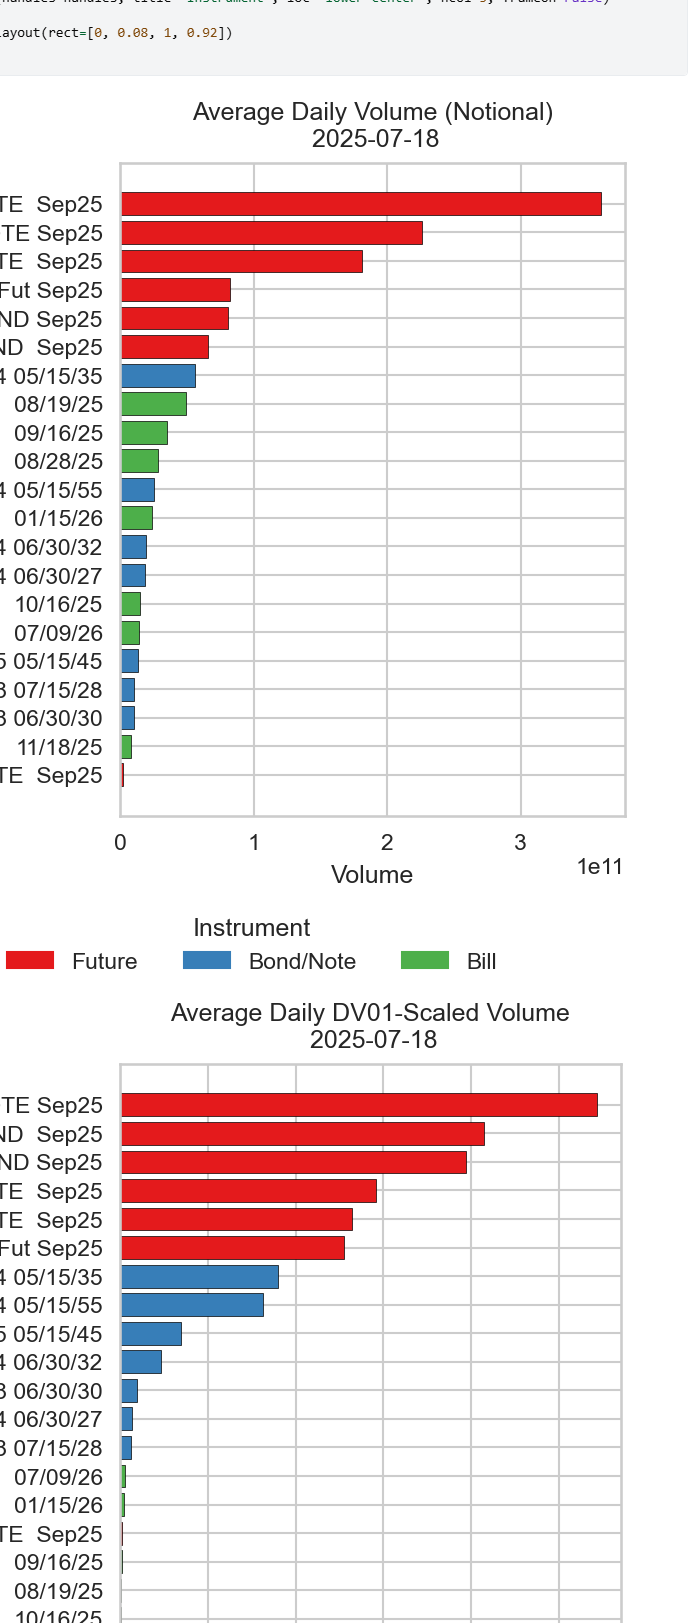
\includegraphics[width=0.9\linewidth,height=0.8\textheight,keepaspectratio]{figures/L4_2_c09_volume_zoom.png}\end{center}
Side-by-side bars of notional volume (top) and DV01-scaled volume (bottom)
by instrument; red bars are exchange-listed futures across the duration
grid, blue and green bars are individual Treasury CUSIPs. On the
DV01-scaled measure (bottom panel), the 10-year, Ultra Bond, Long Bond,
5-year, and 2-year futures all beat every individual cash Treasury except
the most recent few on-the-run notes.
\end{keyblock}

The lecturer opened by contrasting the cash and futures markets directly,
reusing the September-markets intuition: futures contracts aggregate
liquidity across a whole maturity bucket into a single exchange-traded
contract, whereas the cash market splits that liquidity across dozens of
CUSIPs --- the four years leading up to a given maturity date each have
several bills, notes, and off-the-run issues, and no single one of them is
especially liquid. A hedger who wants to short a five-year exposure can
either pick one on-the-run five-year note (limited size, narrow bid-ask)
or short one FVM5 future (all the 5-year liquidity on the exchange
collected in one ticker). The second option is almost always easier.

\begin{tipblock}
\textbf{Filling the gap.} The DV01-scaled measure is notional $\times$
modified duration, so it expresses risk transferred per day rather than
face exchanged per day. The reason this matters: a 30-year Long Bond and a
2-year Note at the same notional volume transfer very different amounts of
interest-rate risk. The DV01-scaled chart is the honest comparison for a
trader sizing a hedge --- \emph{how much interest-rate exposure am I
actually shuffling?} --- and it is the measure on which futures beat the
cash market even more decisively than on raw notional.
\end{tipblock}

\subsection{The deliverable basket and conversion factors}\label{L4-sec:tf-basket}

\begin{keyblock}
\textbf{Cells~12--26.} \emph{Delivery, Pricing, and CTD.}\\
In order to increase liquidity, a Treasury futures contract allows
delivery of a range of Treasury notes or bonds, not a single specific
issue. The 10-year futures contract (TY, now TN / Ultra-10) contains
optionality with regard to which Treasury note can be delivered: any U.S.
Treasury note with remaining maturity between $6.5$--$10$ years. The
reason to broaden the basket is to prevent a short from being squeezed
against a single issue that happens to be scarce at delivery.

\textbf{Conversion factors.} The deliverable bonds differ in maturity and
coupon, and the exchange publishes a \emph{conversion factor} $\phi^i$
for each eligible bond $i$. At delivery, the futures settlement price
$\mathcal{F}(T,T)$ is multiplied by $\phi^i$ to determine the cash the
short receives for delivering bond $i$:
\[
  \text{delivery invoice} \;=\; \phi^i\,\mathcal{F}(T,T) + A^i_T,
\]
where $A^i_T$ is accrued interest on bond $i$.

\textbf{Example: FVM5 (5-year T-Note, June 2025 delivery).} On
2025-02-25 the data file lists the seven eligible notes; each has a
conversion factor in the 0.90--0.94 range, reflecting that most of the
deliverable 5-year notes carry a 3.5--4.4\% coupon against the 6\%
published assumption.
\end{keyblock}

The lecturer walked the class through this carefully, because the
conversion-factor idea is deeply non-obvious. Think of the contract as a
long-short auction: the exchange wants a short to be indifferent (at
settlement) between delivering any two bonds in the basket, so that the
short's optionality does not translate into a settlement lottery. The
conversion factor is the exchange's attempt to make that indifference hold
when the basket is evaluated at a single reference rate.

The factor for bond $i$ is computed by pricing bond $i$ at a flat 6\% yield
and dividing by its face,
\[
  \phi^i \;=\; \frac{1}{100}\sum_{j=1}^n \frac{c_i/2}{(1+.06/2)^{2T_{ij}}}
                \;+\; \frac{1}{(1+.06/2)^{2T_{in}}},
\]
where the sum runs over the coupon dates of bond $i$ remaining at the
delivery date. The lecturer walked through why each ingredient is chosen
the way it is.

\emph{Why a single flat rate, and why 6\%?} A single reference rate is the
only way to get a published, immutable conversion factor: the exchange
needs a $\phi^i$ it can print at contract issue and never revise. Using
``today's'' rate (a spot curve or YTM) would make $\phi^i$ move with the
market and defeat the whole purpose of a conversion factor. The specific
value 6\% is the rate the CME used historically when rates were higher;
they left it in place through the low-rate era because it is
\emph{immutable} for each outstanding contract. When the exchange rolls a
new generation of contracts it can change the convention, but the existing
tickers run to expiry on the old rule. The lecturer answered a student
question about whether 6\% was meaningful with ``I mean, I have no idea,
and it really doesn't matter. They just put in any number there.''

\emph{Does the 6\% miscalibration matter?} Because the actual spot curve
is much lower than 6\% (``closer to 4\%'' in 2025), the convention
uniformly \emph{undervalues} every bond in the basket. The lecturer
pressed the class on whether that mattered, and walked them to the
answer: no, because the short picks the cheapest-to-deliver bond and the
relative ranking of bonds is what drives the short's decision. A uniform
undervaluation shifts every delivery price by approximately the same
amount and leaves the CTD ranking unchanged. It also means that $\phi^i$
for a bond whose coupon is below 6\% sits below 1 (demerit); above 6\%
sits above 1 (credit); at 6\% sits exactly at 1. The \$100 face receives
the credit or demerit as a multiplicative scaling --- ``so in some ways you
could say they could look at maybe the yield to maturity. Don't we already
have a metric for that?'' The lecturer's answer to his own question was
that YTM depends on \emph{price}, which is real-time, so using YTM would
make the conversion factor move every second. Present value at a flat 6\%
is the cleanest rule that uses only coupon and maturity.

\begin{tipblock}
\textbf{Filling the gap.} The factor-1 bond is by construction the bond
whose cashflows, when present-valued at 6\%, equal face. For a freshly
issued Treasury this requires coupon $\approx$~6\% and maturity matched to
the contract window. The exchange does not need any such bond to exist in
the basket --- $\phi^i$ is well-defined for each actual deliverable --- but
this observation is useful for sanity-checking the numbers: if two bonds
in the basket have nearly equal coupon and maturity, their $\phi^i$ must
be nearly equal, and the CTD choice between them will be driven by the
cash-market price differential alone.
\end{tipblock}

\subsection{Delivery cost, gross basis, and net basis}\label{L4-sec:tf-basis}

\emph{(Audio gap begins here. The lecturer was working through cells~27--46
of 4.2, ``Gross and Net Basis,'' for the next 45 minutes. The prose below
reconstructs the teaching order from the frames and the cell content; the
formulas are exactly as stated on the live page.)}

\begin{keyblock}
\textbf{Cells~27--35.} \emph{Gross and Net Basis.}\\
\textbf{The basis trade.} Being long the bond's basis means taking a
position of:
\begin{itemize}
  \item long a \emph{forward} bond at the delivery date $T$, financed spot
        via term repo;
  \item short the corresponding futures contract, adjusted by the
        conversion factor.
\end{itemize}

\textbf{Gross basis} measures the basis trade where the bond is transacted
\emph{spot} (no forward), and the futures leg is unadjusted for carry:
\[
  B^i_{t,t+\tau} \;=\; P^i_t \;-\; \phi^i\,\mathcal{F}(t,T).
\]

\textbf{Net basis} measures the same trade but with the spot leg replaced
by a \emph{forward} bond, so it absorbs the carry:
\[
  \tilde B^i_{t,t+\tau} \;=\; P_{\text{fwd}}^i(t,T) \;-\; \phi^i\,\mathcal{F}(t,T).
\]

\textbf{Alternate view.} Since the forward drop equals the bond's carry,
$\tilde B$ can be read as $B^i - \text{carry}$: net basis is gross basis
minus the carry over the contract horizon.
\end{keyblock}

The conceptual shape of the basis trade follows directly from the forward
identity of~\S\ref{L4-sec:fwd-carry}. If the forward price were the only
no-arbitrage price for a Treasury on the delivery date, then after the
conversion-factor adjustment the futures price $\mathcal{F}(t,T)$ would
equal $P_{\text{fwd}}^i(t,T)/\phi^i$ for the CTD bond, and the net basis
for the CTD would be identically zero. The basis trade is the wager that
this equality is \emph{nearly but not exactly} right, and that the
relative ordering of basis values across the deliverable basket tells you
which bond the short will elect to deliver.

The split between gross and net basis matters because Wall Street quotes
the trade in net basis even though it transacts the spot leg: the
quoted number is already carry-adjusted, so a zero gross basis does not
mean a zero-P\&L trade. A trader who pays the gross basis to go long
collects the carry until delivery, and the carry is the \emph{majority}
of the P\&L on most basis trades. The lecturer emphasized this enough on
the live page that the \emph{Alternate View} callout exists precisely to
head off the confusion.

\begin{keyblock}
\textbf{Cells~36--41.} \emph{Examples: Gross and Net Basis (FVM5, 2025-02-25).}\\
\begin{center}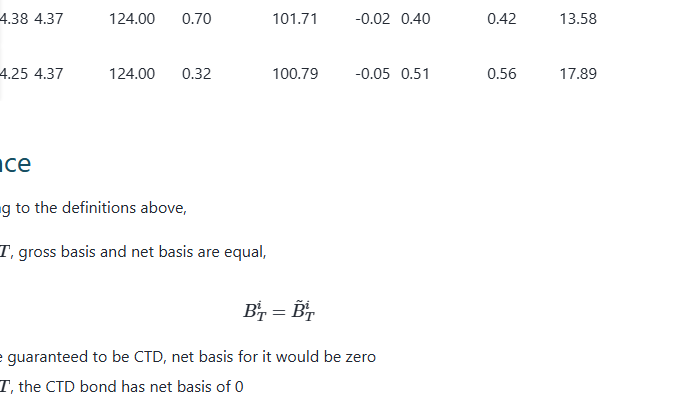
\includegraphics[width=0.9\linewidth,height=0.8\textheight,keepaspectratio]{figures/L4_2_c41_net_basis.png}\end{center}
Bond-by-bond table of coupon, repo rate, days to forward, accrued interest,
dirty price, carry, gross basis, and net basis across the deliverable
basket. All seven bonds share a common $r_{\text{repo}} = 4.37\%$ and a
$124$-day forward interval. Net basis ranges from $+0.07$ (for the
91282CLK 2029-08-31 note) to $+0.56$ (for the 91282CMG 2030-01-31 note) ---
all positive, with the smallest belonging to the CTD.
\end{keyblock}

The student is meant to spot two things in this table. First, net basis is
positive for every bond in the basket: the short's option to select among
bonds extracts a non-zero premium from the long, so the basis trader
\emph{pays} rather than collects this value. Second, the CTD (here 91282CLK)
has the smallest net basis --- not zero, because of the embedded optionality
of~\S\ref{L4-sec:tf-options}, but the smallest among the deliverables. Any
long-CTD / short-future trade earns the carry over the contract horizon and
loses the option premium the short keeps.

\begin{keyblock}
\textbf{Cells~42--46.} \emph{Convergence and caveats.}\\
\textbf{Convergence.} At expiration $T$, gross basis and net basis are
equal ($B^i_T = \tilde B^i_T$, because carry over zero time is zero) and
for the CTD both are zero:
\[
  B_T^{\text{CTD}} \;=\; \tilde B_T^{\text{CTD}} \;=\; 0.
\]

\textbf{Importance of Net Basis.} Net basis is the most commonly quoted
measure because it strips out the predictable carry component and isolates
the trader's bet on the optionality.

\textbf{Daily settlement.} The P\&L of the basis trade as above is only
approximate: daily settlement on the short-futures leg produces
intermediate cashflows that the forward-bond leg does not mirror,
contributing a (usually small) timing wedge.

\textbf{Repo caveat.} The synthetic forward relies on \emph{term} repo
over the contract horizon. In practice, term repo for $\tau$ months may
not be deep enough to fund the position; the trader may have to roll
overnight repo, accepting daily re-pricing of the financing rate.
\end{keyblock}

The two caveats are worth pausing on because they explain why basis
trading is its own desk. Daily settlement means the short leg receives or
pays cash every day, which must be invested or borrowed; the forward leg
has no such cashflow. In a rising-rate environment, the short leg receives
cash on down days and reinvests at the higher new rate, giving the short
a small positive bias; the basis trader has to mark this correction
against the quoted basis when comparing actual to theoretical P\&L. The
repo caveat reminds the trader that the forward-leg construction is an
approximation: term repo is often thin beyond a few weeks, so the
synthetic forward may be reconstructed nightly from overnight repo, with
each roll marked at the prevailing overnight rate. If the repo rate
spikes (as in the September 2019 repo crisis, referenced in
\S\ref{L4-sec:swap-spread-pointer}), the basis trade can be swamped by
financing costs.

\subsection{Implied repo}\label{L4-sec:tf-impliedrepo}

\begin{keyblock}
\textbf{Cells~47--55.} \emph{Implied Repo.}\\
The \textbf{implied repo rate} for bond $i$ is the repo rate that
rationalizes the ``futures-as-forward'' relationship:
\[
   F(t,T)^i \;=\; \mathcal{F}(t,T)\,\phi^i.
\]
Solve for $r^i_{\text{IR}}$ from
\[
   \underbrace{F(t,T)^i + A^i_T}_{\text{dirty forward}}
     \;=\; \underbrace{\bigl[P^i_t + A^i_t\bigr]}_{\text{dirty spot}}
        \bigl[1 + r^i_{\text{IR}}\,\tau_{\text{act}/360}\bigr],
\]
where $r^i_{\text{IR}}$ is the implied repo rate on bond $i$ and
$\tau_{\text{act}/360}$ is the forward interval in years under the
ACT/360 money-market convention.

\textbf{Trading-strategy interpretation.} $r^i_{\text{IR}}$ is the
annualized return from a trader who at time $t$:
\begin{itemize}
  \item buys bond $i$ spot;
  \item shorts the futures contract (with conversion factor $\phi^i$);
  \item holds both to delivery and delivers bond $i$ into the short.
\end{itemize}
If bond $i$ does end up being CTD, $r^i_{\text{IR}}$ is the trader's
realized return. If bond $i$ is \emph{not} CTD, the trader finds that
the price of the (now suboptimal) long-delivery is compromised relative
to the CTD, and the realized return is less than $r^i_{\text{IR}}$.

\textbf{Careful: this implied repo is assuming the bond becomes CTD!} A
high implied repo rate may simply mean the bond is unlikely to become
CTD (so the calculation is based on a counterfactual) rather than a
genuine arbitrage opportunity.
\end{keyblock}

The interpretation the lecturer drives home on this page is the third
bullet: $r^i_{\text{IR}}$ is not a universal ``repo rate implied by the
futures chain'' but a \emph{bond-by-bond} quantity that tells the trader
how much they would earn if they locked in bond $i$'s futures-to-spot
spread through delivery. The trader cannot actually earn $r^i_{\text{IR}}$
on any bond of their choice, because the short-futures leg pays off at
$\phi^{\text{CTD}}\mathcal{F}(T,T)$ regardless of which bond the trader
holds.

\begin{tipblock}
\textbf{Filling the gap.} There is a clean relationship between implied
repo and the CTD rule:
\[
   i^\star \;=\; \arg\max_i r^i_{\text{IR}}.
\]
The bond with the highest implied repo is (by definition) the bond
delivering the highest annualized return through the synthetic-forward
calculation, which is exactly the bond the short would choose to deliver.
A table of implied repo rates ranked across the basket is therefore a
direct CTD screen: the highest number is the short's best choice. The
convenience of ranking by a single annualized number is why desks quote
implied repo alongside net basis --- they carry the same information in
different units, but implied repo is dimensionless (a rate) where net
basis is in dollars.
\end{tipblock}

\subsection{The cheapest-to-deliver computation}\label{L4-sec:tf-ctd}

\begin{keyblock}
\textbf{Cells~56--65.} \emph{Cheapest to Deliver.}\\
\textbf{Conversion factor.} $\phi^i$ is the publicly published, immutable
scaling of the delivery price of bond $i$ at the reference rate of 6\%.

\textbf{Delivery cost.} For a short position, the cost to deliver bond
$i$ to close out the futures contract is
\[
   \text{delivery cost}_T \;=\; \bigl(P^i_T + A^i_T\bigr)
                               \;-\; \bigl(\phi^i\,\mathcal{F}(T,T) + A^i_T\bigr)
                           \;=\; P^i_T \;-\; \phi^i\,\mathcal{F}(T,T).
\]
Accrued interest cancels, so the delivery cost is simply the bond's price
(clean or dirty, they differ by the same $A^i_T$ that cancels) minus the
converted futures price.

\textbf{CTD rule.} Shorts choose to deliver the bond that minimizes
delivery cost:
\begin{align*}
   \text{CTD} &\;=\; \arg\min_i \bigl[P^i_T - \phi^i\,\mathcal{F}(T,T)\bigr] \\
              &\;=\; \arg\min_i \frac{P^i_T}{\phi^i},
\end{align*}
where the second equality holds because $\mathcal{F}(T,T)$ is the same
across all bonds in the basket --- it factors out.

\textbf{Convergence at expiry.} By no-arbitrage, at expiry,
\[
   \mathcal{F}(T,T) \;=\; \frac{P^{\text{CTD}}_T}{\phi^{\text{CTD}}}
                       \;\le\; \frac{P^i_T}{\phi^i} \quad \forall i.
\]

\textbf{Example: CTD Determination.} Bloomberg identifies the CTD Treasury
note along with its gross and net basis.
\begin{center}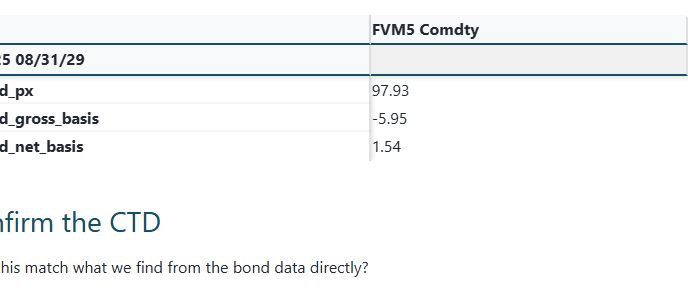
\includegraphics[width=0.7\linewidth,height=0.25\textheight,keepaspectratio]{figures/L4_2_c62_bbg_ctd.png}\end{center}
The contract (FVM5 Comdty) shows CTD price $97.93$, gross basis $-5.95$,
and net basis $+1.54$.

\textbf{Confirm the CTD.} Computing $P^i_T - \phi^i\,\mathcal{F}(T,T)$
directly from the bond data for all seven deliverables produces a
delivery-cost column whose minimum flags the CTD.
\begin{center}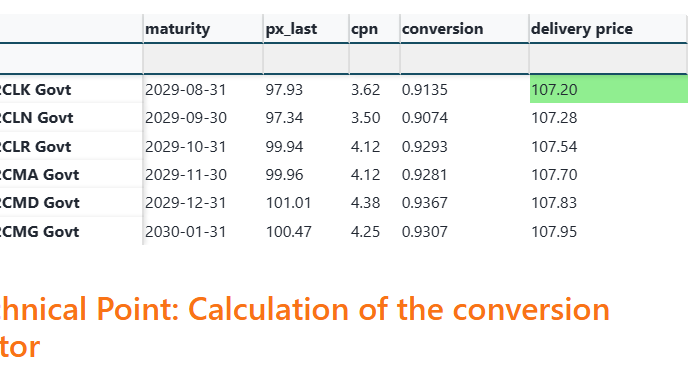
\includegraphics[width=0.9\linewidth,height=0.6\textheight,keepaspectratio]{figures/L4_2_c65_confirm_ctd.png}\end{center}
The $91282\mathrm{CLK}$ note (2029-08-31, 3.62\% coupon, $\phi = 0.9135$)
has delivery cost $107.20$, the smallest in the basket --- highlighted in
green as the CTD. The worst candidate, 91282CMG (2030-01-31, 4.25\%), has
delivery cost $107.95$ --- only 75 cents worse, but on a standardized
futures contract that 75 cents is the short's option value.
\end{keyblock}

The \emph{convergence at expiry} identity is the single most important
equation on this page. Before expiry, $\mathcal{F}(t,T)$ is set by the
market; at expiry, the futures price must converge to the price/phi ratio
of whichever bond the short chooses --- and the short chooses to minimize
that ratio. The intuition is the arbitrage argument: if at expiry the
futures price exceeded any bond's $P^i_T/\phi^i$, the short could buy bond
$i$ in the cash market, deliver it into the short-future, and collect the
difference risk-free; the short's demand drives $\mathcal{F}(T,T)$ up to
the cheapest ratio.

The \emph{minimization in delivery cost = minimization in price/phi ratio}
equivalence is why Bloomberg's quoted ``CTD'' column is computed by
ranking the delivery-cost column, not by computing the price/phi ratio
directly: the two rankings agree by construction, and the delivery-cost
column is what traders actually compute at expiry.

\begin{keyblock}
\textbf{Cell~66.} \emph{Technical Point: Calculation of the conversion factor.}\\
Suppose bond $i$ has coupon rate $c_i$ and $n$ coupon periods remaining at
delivery. Its conversion factor is
\[
   \phi^i \;=\; \frac{c_i}{.06}\Bigl(1 - \frac{1}{(1+.06/2)^{2T_{in}}}\Bigr)
              \;+\; \frac{1}{(1+.06/2)^{2T_{in}}}.
\]
(This is the standard present-value formula for an annuity of $c_i/2$
coupon payments plus a 1-of-face principal repayment, discounted at 6\%
semiannual compounding.) Note that $\phi^i$ is constant over the length of
the futures contract; there is no time subscript. The formula depends
only on bond $i$'s coupon rate and its remaining maturity at the contract
delivery date.
\end{keyblock}

\begin{keyblock}
\textbf{Cell~67.} \emph{Understanding CTD.}\\
\textbf{In a low-rate environment} (such as 2008--2021): \emph{lower-coupon,
shorter-maturity} bonds tend to be CTD, because $\phi^i$ shrinks below 1
by less for these bonds under the 6\% convention, and their cash prices
are relatively higher than the 6\%-convention valuations would predict.

\textbf{In a high-rate environment}: \emph{higher-coupon, longer-maturity}
bonds tend to be CTD --- the same mechanism running in reverse.
\end{keyblock}

The CTD story is sensitive to the \emph{difference} between the actual rate
and the 6\% convention. When actual rates are well below 6\% (the norm
2008--2021), the convention undervalues every bond; the degree of
undervaluation is larger for longer maturities (the discount factor
mismatch accumulates), so the conversion factor shrinks more for long
bonds than the market price does, which makes long bonds \emph{more}
expensive to deliver per unit of conversion. The rule of thumb is that
when rates are low, the CTD rotates to the short end of the basket; when
rates are high, it rotates to the long end.

\subsection{Embedded optionality}\label{L4-sec:tf-options}

\begin{keyblock}
\textbf{Cells~68--77.} \emph{Embedded Optionality of Treasury Futures.}\\
Bond futures embed several options that belong to the \emph{short}:
\begin{itemize}
  \item Quality option.
  \item Timing option.
  \item End-of-Month option.
  \item Wildcard option.
\end{itemize}
These options collectively explain why the CTD's net basis is positive
rather than zero; the long pays the short for the package of delivery
flexibilities.
\end{keyblock}

\paragraph{Quality option.} The short chooses which bond from the basket to
deliver. Formally, each bond's delivery cost $P^i_T - \phi^i\mathcal{F}(T,T)$
can flip sign or ordering between the trade date and the expiry date, and
the short extracts the minimum. The value of this option is proportional
to the dispersion of bond-level characteristics in the basket (wider
maturity range, wider coupon range $\Rightarrow$ more option value). Large
quality-option value arises in high-rate or high-volatility environments,
because the CTD rotation becomes more responsive to rate moves.

\paragraph{Timing option.} The short may deliver on \emph{any day} of the
delivery month, not only the last. This is the key content of the
``collect carry'' versus ``retain option value'' bullet on the slide.

\begin{keyblock}
\textbf{Cell~75.} \emph{Timing Option.}\\
\begin{itemize}
  \item If coupon is \textbf{higher} than repo, deliver \textbf{late} as
        possible:
        \begin{itemize}
          \item collect carry;
          \item retain option value.
        \end{itemize}
  \item If coupon is \textbf{lower} than repo, delivery is \textbf{ambiguous}.
        Early delivery would:
        \begin{itemize}
          \item eliminate negative carry;
          \item eliminate option value.
        \end{itemize}
\end{itemize}
It is a quantitative issue whether forfeiting the option value is worth
eliminating the negative carry.
\end{keyblock}

The trade-off is mechanical. When coupon $>$ repo, the short's ongoing
position has positive carry --- each day the short holds the bond, coupon
accrual exceeds financing cost, so delaying delivery is profitable. In
this regime the short delays to the last possible day and keeps the
option to switch bonds along the way. When coupon $<$ repo, holding the
bond costs money (negative carry), so the short has an incentive to
deliver early; but delivering early gives up the option to switch to a
different CTD if rates move in the interim. The lecturer's slogan --- ``a
quantitative issue whether forfeiting the option value is worth
eliminating the negative carry'' --- is the resolution: the short computes
the present value of expected future option rotations against the present
value of daily negative carry, and delivers when the balance flips.

\paragraph{End-of-Month option.} Contract trading ends roughly three weeks
into the delivery month, but the short retains another week before the
final delivery date. The futures price is pinned by the final-trade-day
settlement, but bond prices continue to move over the intervening week,
giving the short an additional sliver of time to re-optimize the CTD
choice.

\paragraph{Wildcard option.}
\begin{keyblock}
\textbf{Cell~77.} \emph{Wildcard Option.}\\
\begin{itemize}
  \item Trading on the exchange settles at 2pm CT yet the shorts have a
        few more hours to decide whether to issue a notice of delivery.
  \item Thus, a basis trade long the CTD and hedged with futures will
        consider a post-settlement change in CTD price:
        \begin{itemize}
          \item The seller might decide to deliver if the price of the
                CTD moves favourably between the time the exchange settles
                to $F_t$ but before delivery notice is due.
        \end{itemize}
  \item This is like the timing option --- a question of whether the
        moneyness outweighs the ongoing option value.
\end{itemize}
\end{keyblock}

The wildcard is the subtlest of the four. At 2:00pm Central time the
futures contract settles for the day at a final price $F_t$ --- no further
trades are marked against that day's contract. But the physical market for
the underlying bonds continues to trade for another two hours, and the
short's decision to issue a delivery notice is not due until 6:00pm. If
between 2:00pm and 6:00pm the CTD's cash price drops, the short can
\emph{buy} the CTD in the cash market at the lower price and deliver into
the 2:00pm-locked futures settlement at the higher price. The short
collects a risk-free (within the 2:00-6:00 window) profit. This is a
genuine free option --- the short pays nothing for it --- and its value
scales with the volatility of the CTD's afternoon price drift.

\begin{checkpoint}
\textbf{My note.} The four options look baroque but they all follow the
same principle: \emph{the short gets to observe state before committing to
a decision}, where the ``decision'' is some aspect of delivery (which
bond, what day, what intraday moment). The long bought a contract that is
indifferent across all these choices, and pays for the short's observation
value. Quantitatively, all four option values rise with the volatility of
the underlying (more state variation $\Rightarrow$ more to observe) and
with the length of the delivery window (more decisions to make). In
low-volatility, short-window environments, the embedded options are
nearly worthless and the CTD's net basis is close to zero; in
high-volatility, month-long-delivery environments, the CTD's net basis
is several ticks positive and is the lecturer's recurring answer to
``why doesn't the quoted basis converge to zero before expiry?''
\end{checkpoint}

\section{Swaps}\label{L4-sec:sw}

\emph{(Audio returns around 85:30 mid-sentence --- ``interest rate swap,
what is it?'' The lecturer has already scrolled through the first two
cells of \emph{5.1.~Swaps} (Size of the market, Definition) during the
audio-gap tail; the transcript picks up at the first fixed-for-floating
discussion.)}

\subsection{Size of the swap market}\label{L4-sec:sw-size}

\begin{keyblock}
\textbf{Cells~2--7.} \emph{Size of Swap Markets.}\\
\textbf{Global OTC derivatives (end-2024):}
\begin{center}
\begin{tabular}{lrr}
\toprule
\textbf{Product} & \textbf{Notional (\$T)} & \textbf{Gross MV (\$T)} \\
\midrule
Interest Rate Swaps     & 446.9 & 10.6 \\
Forward Rate Agreements &  55.1 & 0.5  \\
Interest Rate Options   &  46.2 & 0.4  \\
Equity Options/Derivs   &   8.9 & 0.4  \\
\bottomrule
\end{tabular}
\end{center}
\begin{center}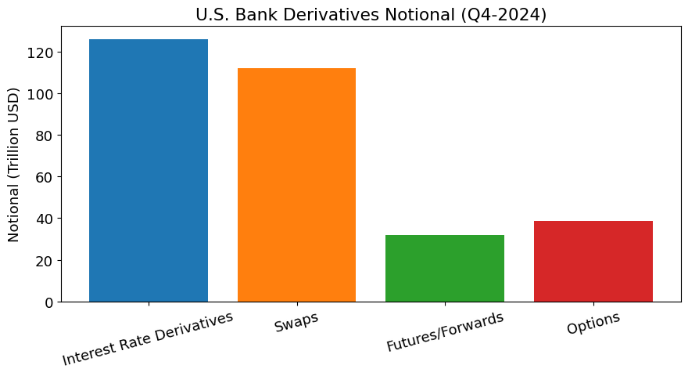
\includegraphics[width=0.9\linewidth,height=0.6\textheight,keepaspectratio]{figures/L5_1_c06_otc_products.png}\end{center}
U.S. bank derivatives notional (Q4-2024): interest rate derivatives and
swaps together account for more than four-fifths of the notional;
futures/forwards and options are each under~\$40T.

\textbf{Sources.} Bank of International Settlements and OCC Quarterly
Report (Q4~2024).
\end{keyblock}

The lecturer's opening point on \emph{5.1} is that the swap market is not
just large, it is \emph{larger than the government-bond market combined
with every other fixed-income instrument on an exchange}. The BIS
end-2024 notional of $\$447$T in interest-rate swaps dwarfs every
cash-bond market; it is an order of magnitude larger than the global
futures notional and two orders larger than the equity-derivatives
notional. The gross market value column tells a different story --- $\$10.6$T
in IRS is small relative to the $\$447$T notional because most
outstanding swaps have net-present value close to zero (see the ``no cost
to initiate'' property below), so the gross exposure is a tiny fraction
of the notional.

\begin{tipblock}
\textbf{Filling the gap.} Notional and gross market value answer different
questions. Notional is the \emph{reference} quantity on which interest
accrues; gross market value is the \emph{replacement cost} of the swap
to one of the two counterparties (sum of positive MTMs across all
outstanding contracts). A swap written at market has zero gross market
value on day one and accumulates $|V_{\text{sw}}|$ as rates move. The
ratio (gross market value / notional) $\approx 2.4\%$ for IRS is a rough
proxy for the average cumulative P\&L swing across all outstanding swaps
--- small in percentage terms, but $\$10.6$T in dollars, which is why
regulatory collateral is a non-trivial share of bank balance sheets.
\end{tipblock}

\subsection{Definition and fixed-for-floating mechanics}\label{L4-sec:sw-def}

\begin{keyblock}
\textbf{Cells~8--15.} \emph{Definition; Fixed-for-Floating; Swap Rate; Specifications.}\\
A \textbf{swap} works as follows:
\begin{itemize}
  \item Two counterparties agree at $t$ to swap payments on future dates.
  \item The payments may be based on fixed vs.~floating interest rates on
        the same currency, or fixed rates across two currencies.
  \item The swap designates a \textbf{notional} base for the interest
        rates, but the notional is not exchanged.
\end{itemize}

\textbf{Fixed-for-floating.} A fixed-for-floating interest-rate swap is an
agreement with the following obligations:
\begin{itemize}
  \item Party A pays a fixed rate $c_{\text{sw}}$ on the notional each
        payment date;
  \item Party B pays a floating rate (typically SOFR) on the notional,
        observed at each reset date.
\end{itemize}

\textbf{Swap rate.} The fixed rate in the fixed-for-floating swap,
$c_{\text{sw}}$, is the \emph{swap rate}. It is set at initiation so that
the PV of the two legs is equal.

\textbf{Specifications.}
\begin{itemize}
  \item Frequency: floating often quarterly, fixed often semiannual.
    (Post-LIBOR SOFR swaps often move to annual on the fixed leg.)
  \item Floating rate: SOFR (post-2022); LIBOR (pre-2022, now retired).
  \item Day count: ACT/360 on the floating leg, ACT/365 or 30/360 on the fixed.
\end{itemize}

\textbf{No cost to initiate.} Like a forward, there is no price to enter a
swap; the swap rate is chosen such that the contract has zero value at
$t=0$. Value accrues only as floating rates diverge from the initial swap
rate.

\textbf{Example: SOFR swap.} Pay fixed $c_{\text{sw}}$ on \$1M notional,
receive SOFR on \$1M notional; both legs quarterly. The lecturer walked
through this on the board with a student-partner exchange --- one student
plays the fixed-paying bank, the lecturer plays the floating-paying
counterparty.
\end{keyblock}

Once the microphone came back, the lecturer started by picking a
student and building up the swap definition from scratch. The question was
``an interest rate swap --- what is it?'' and the student's answer
(``fixed leg pays a fixed amount, floating leg pays whatever's prevailing
in the market, usually LIBOR or SOFR'') was the right summary. The
lecturer pushed on the LIBOR point: LIBOR is retired in the U.S. (``LIBOR
is gone''), so the modern fixed-for-floating swap is a SOFR-for-fixed
swap --- the same two overnight-rate benchmarks introduced in Lecture~3,
running in the dominant direction.

The lecturer then walked the class through a concrete example: a
\$1M-notional SOFR-for-fixed swap. ``I'm going to pay you SOFR on a
notional of a million dollars --- am I actually paying him a million
dollars? Absolutely not. He's never going to touch the million. But I'm
going to pay SOFR on some million dollars.'' The lecturer underlined
\emph{notional is not exchanged} as the single-most-important
misconception; the notional is just the reference against which the rate
applies. When SOFR is 4\% annualized, the quarterly floating payment on
\$1M notional is $\$1{,}000{,}000 \cdot 0.04/4 = \$10{,}000$ per quarter.

The lecturer's standard ``how often do we pay?'' prompt got the usual
mixed answer (semiannual, quarterly). In LIBOR days, the floating
(variable) side paid quarterly and the fixed side paid semiannually --- ``a
mess.'' In SOFR-swap days, both legs typically pay annually on the same
date: ``nice and easy.'' For the example, he picked annual payments at the
end of each of ten years.

\begin{keyblock}
\textbf{How do we set $c_{\text{sw}}$?} The fixed rate must be chosen such
that the swap has zero value at $t=0$. Three candidate rules are on the
table:
\begin{enumerate}
  \item Pick ``SOFR right now'' --- a known quantity, easy to quote.
  \item Pick an average of market expectations over the contract horizon.
  \item Pick the rate at which the market is \emph{willing to enter the
        swap} --- i.e., observed from other live swaps.
\end{enumerate}
\end{keyblock}

The student's first instinct was (1): use today's SOFR as the fixed rate.
The lecturer accepted it but pushed back: ``I don't love it because, you
know, what if the market has a strong view rates are going down over the
ten years? Then, well, I would actually love it because you're going to
lock in at that, but you shouldn't love it.'' In other words: option~(1)
is simple but asymmetric --- whoever has the better view of the rate path
will prefer one side, which breaks the no-cost-to-initiate property.

The lecturer then moved to (2): an average of market expectations. Where
would we get this? ``Yield curve, though there's a term premium in there,
but also STIR futures. That's going to give me a pretty clear idea on
what the market expects SOFR to do for the next 18 months.'' STIR futures
(from Lecture~3) are the cleanest source of the market's SOFR expectation
through the FFF/SOFR-futures chain. Over a 10-year horizon the futures
chain is not deep enough, but the expectations measure still underlies
the cleanest theoretical answer: $c_{\text{sw}}$ is the PV-weighted
average of expected SOFR rates over the contract horizon.

The third option, (3), is what the market actually does. ``This swap
market is going to function at very high liquidity, massive volumes. We're
going to come in, we're going to look at the data, and say \emph{that} is
an excellent place to source some data on what the market must be
expecting.'' In other words: the swap market \emph{defines}
$c_{\text{sw}}$ by auction, and swap-rate quotes on the Bloomberg screen
are the consensus answer to the expectations question. The swap-rate
formula below is the theoretical no-arbitrage identity that connects
(3) back to the spot-discount curve.

\subsection{Swaps as bonds, swaps as forwards}\label{L4-sec:sw-asbonds}

\begin{keyblock}
\textbf{Cells~16--18.} \emph{Swaps, Forwards, and Floaters.}\\
\textbf{Swap as bonds.} A fixed-for-floating swap can be replicated with
fixed-rate and floating-rate bonds:
\begin{itemize}
  \item Receive fixed $\Leftrightarrow$ long a fixed-rate bond + short a
        floating-rate note (FRN).
  \item Pay fixed $\Leftrightarrow$ short a fixed-rate bond + long a FRN.
\end{itemize}
The notionals cancel, leaving exactly the pattern of fixed and floating
interest payments that the swap exchanges.

\textbf{Swap as forwards.} A forward contract can be seen as a
single-date swap. Thus, a multi-date swap is a \emph{portfolio of
forwards}, each settling at one of the swap's payment dates.
\end{keyblock}

The lecturer used the swap-as-bonds identity to motivate the swap-value
formula in~\S\ref{L4-sec:sw-value}. The fixed-rate bond is a conventional
coupon bond paying $c_{\text{sw}}$ on notional; the FRN is the
construction from Lecture~2 notebook~2.4 (``Floating-Rate Notes''), which
the class reviewed on the final segment of this class --- an FRN pays the
prevailing SOFR rate at each reset, and its price sits at par on every
reset date. Combining a long-fixed-bond and a short-FRN exposure: on each
payment date the holder collects the fixed coupon and pays the floating
coupon; the principals cancel (both legs are the same notional). This is
algebraically identical to receiving fixed in a swap.

The swap-as-forwards identity is more subtle and more important for
pricing: a single swap payment date is equivalent to an FRA (or a
single-date forward) exchanging fixed for floating on that date. A
10-year quarterly swap is therefore a portfolio of 40 FRAs, one for each
quarterly payment date. Pricing the swap is pricing each component FRA,
which in the FRA algebra of Lecture~2 \S\ref{L3-sec:stir} reduces to the
sum of present-valued payments against the spot discount curve. The
swap-rate formula is the closed form of this sum.

\subsection{The swap curve}\label{L4-sec:sw-curve}

\begin{keyblock}
\textbf{Cells~19--34.} \emph{Swap Pricing and the Swap Curve.}\\
On a given date, the quoted swap rate $c_{\text{sw}}(0,T)$ across swap
maturities $T$ forms the \textbf{swap curve}. It is the analogue for
swaps of the yield curve for Treasuries: a snapshot, not a time series.

\textbf{Time series of 10-year swap rate.} Over 2018--2025 the 10-year
SOFR swap rate varied from near zero (2020 COVID era) to above 4\% (2023
peak of the hiking cycle) and back to around 4\% in 2025.
\begin{center}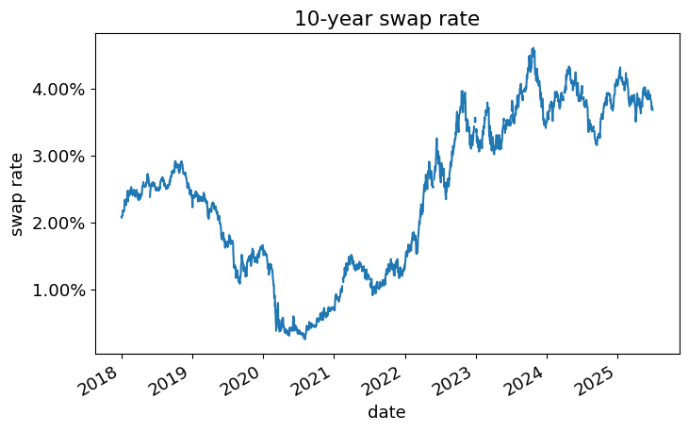
\includegraphics[width=0.8\linewidth,height=0.4\textheight,keepaspectratio]{figures/L5_1_c27_ten_year_ts.png}\end{center}

\textbf{Swap rates move over time, strongly correlated across tenors.}
The multi-tenor overlay (1, 2, 5, 10, 30-year) shows a tight factor
structure; every tenor tracks a common ``level'' factor, with secondary
``slope'' and ``curvature'' deviations.
\begin{center}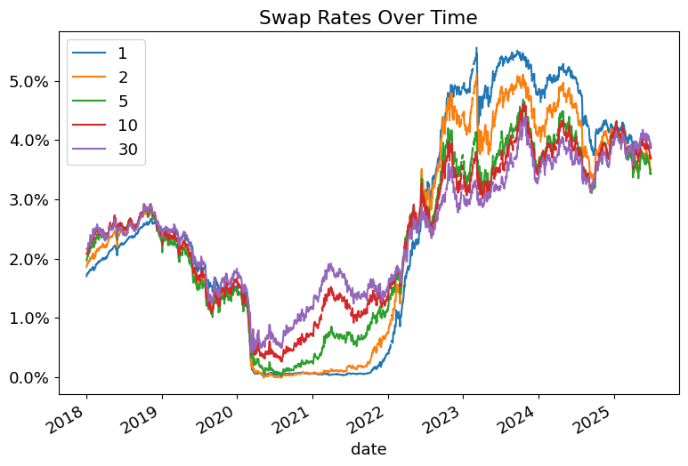
\includegraphics[width=0.8\linewidth,height=0.4\textheight,keepaspectratio]{figures/L5_1_c34_factor_structure.png}\end{center}

\textbf{Swap curves at four snapshot dates.} The swap curve's shape
varies: concave (typical), inverted (2023 hiking cycle), or humped at
short horizons.
\begin{center}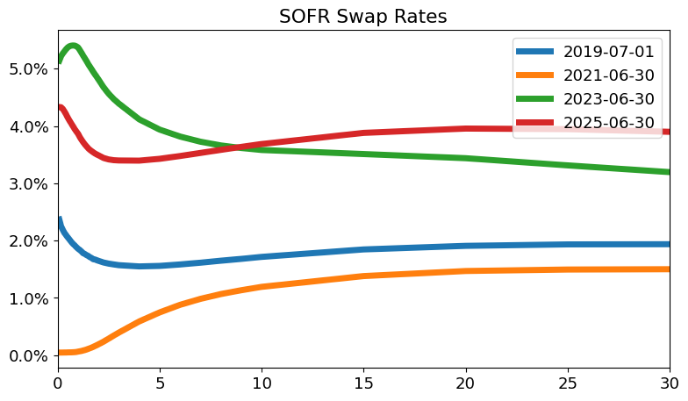
\includegraphics[width=0.8\linewidth,height=0.4\textheight,keepaspectratio]{figures/L5_1_c29_curves_dates.png}\end{center}
The $2019$ curve (blue) is nearly flat around $2\%$; the $2021$ curve
(orange) is sharply upward-sloping from near-zero short rates; the
$2023$ curve (green) is inverted, peaking near $5.5\%$ at the short end
and falling to $3\%$ at $30$ years; the $2025$ curve (red) is downward
sloping from $4.5\%$ to $4\%$, reflecting the market's expectation of
cuts.
\end{keyblock}

The lecturer spent a few minutes walking through the time-series and
curve charts to emphasize that swap rates are \emph{live market data},
not an accounting artifact. The 10-year SOFR swap has been quoted daily
for over a decade; its movements over 2018--2025 are driven by the same
macroeconomic forces as Treasury yields but with a small additive spread
(the \emph{swap spread}, treated below). The factor structure is the same
observation the class saw for Treasury yields in Lecture~1: the first
three principal components of the multi-tenor swap time series account
for $>98\%$ of the variance, and they correspond (in order) to level,
slope, and curvature.

The four-date curve snapshot is instructive for the shape story. In
calm environments (2019), the curve is nearly flat --- the market expects
constant rates indefinitely. In post-shock environments (2021, post-COVID),
the curve steepens sharply as the market prices in an eventual exit from
zero. In tightening environments (2023), the curve inverts --- short rates
higher than long rates, because the market expects a recession-driven
reversal. In mid-cycle environments (2025), the curve is mildly downward
sloping, pricing in a small amount of easing while keeping the front end
near the current policy rate.

\subsection{Swap value and the swap-rate formula}\label{L4-sec:sw-value}

\begin{keyblock}
\textbf{Cells~35--46.} \emph{Swap Value.}\\
The swap's cashflow (from the paying-fixed, receiving-floating side) is
replicated by:
\[
  +\,\text{FRN} \;-\; \text{Fixed bond}.
\]
So the value of paying-fixed is
\[
  V_{\text{sw}}(t,T,c_{\text{sw}})
    \;=\; P_{\text{flt}}(t,T;0) \;-\; P_{\text{fix}}(t,T;c_{\text{sw}}),
\]
where the frequency $m$ and set of payment dates $T_i$ are omitted for
notational simplicity.

\textbf{Implicitly defined swap rate.} $c_{\text{sw}}$ is the value that
makes $V_{\text{sw}}(t,T,c_{\text{sw}}) = 0$ at $t=0$:
\[
   P_{\text{flt}}(0,T;0) \;=\; P_{\text{fix}}(0,T;c_{\text{sw}}).
\]

\textbf{Swap pricing formulas.} Consider a swap with equal frequency $m$
on both legs. A par FRN satisfies $P_{\text{flt}}(0,T;0) = 1$ (face), so
\[
   P_{\text{fix}}(0,T;c_{\text{sw}})
     \;=\; \sum_{i=1}^M \frac{c_{\text{sw}}}{m}\,Z(0,T_i) \;+\; Z(0,T) \;=\; 1.
\]

\textbf{Solving for the swap rate.} Rearranging,
\[
   c_{\text{sw}}(0,T;m)
      \;=\; m\,\frac{1 - Z(0,T)}{\sum_{i=1}^M Z(0,T_i)}.
\]
The notation emphasizes that $c_{\text{sw}}$ depends on the quote date
($0$), the maturity ($T$), and the frequency ($m$) of the swap.
\begin{center}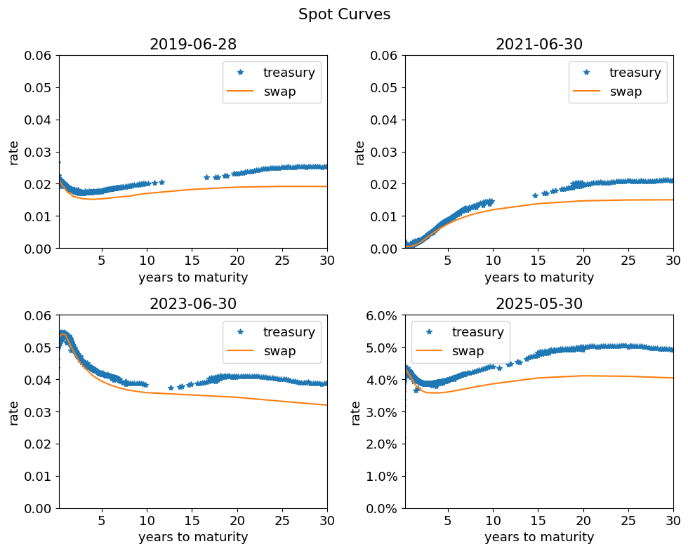
\includegraphics[width=0.9\linewidth,height=0.55\textheight,keepaspectratio]{figures/L5_1_c47_swap_rate_panels.png}\end{center}
Four-panel overlay of Treasury spot curve (blue) and implied swap curve
(orange) across quote dates 2019, 2021, 2023, 2025. The two curves agree
closely, with swap rates tracking or slightly falling short of Treasury
yields.
\end{keyblock}

This formula is the most important content in \emph{5.1}. The
\emph{swap rate is a weighted average of the spot-curve forwards},
weighted by the discount factors at the payment dates. The derivation
uses two mildly non-obvious steps: first, that the floating leg
$P_{\text{flt}}(0,T;0)$ equals par at the quote date (the FRN identity
from \S2.4); second, that the fixed leg at par gives the closed form
above. The lecturer walked through the second step slowly.

\begin{tipblock}
\textbf{Filling the gap.} The floating leg equals par at any reset date
because the coupon payment on the floating leg is \emph{defined} as the
rate required to return the bond to par --- this is the defining property
of an FRN. At a reset date $T_i$, the FRN pays the previous-reset rate on
notional \$1 for the period $[T_{i-1}, T_i]$, which discounted back to
$t = T_i$ gives exactly \$1 --- and no further coupons have been fixed, so
the forward value of the FRN at any future reset date is also \$1. At
initiation ($t=0$, assumed a reset date), the FRN's price is therefore
\$1. Any move of $t$ away from a reset date introduces a small drift due
to the accrued but unfixed portion of the next coupon, but at initiation
the identity is exact.

For the fixed-leg derivation, the closed form comes from:
\[
   \sum_{i=1}^M \frac{c_{\text{sw}}}{m}\,Z(0,T_i) \;=\; 1 - Z(0,T)
   \quad\Longrightarrow\quad
   c_{\text{sw}} \;=\; m\,\frac{1-Z(0,T)}{\sum_i Z(0,T_i)}.
\]
The $1-Z(0,T)$ term is the PV of receiving \$1 of principal plus \$1 of
interest in total (the structure of a par bond); dividing by the sum of
discount factors gives the periodic coupon.
\end{tipblock}

In practice, a trader reads the swap curve off the screen and uses the
formula the \emph{other} way --- not to solve for $c_{\text{sw}}$ given
$Z(\cdot,\cdot)$, but to \emph{imply} $Z(\cdot,\cdot)$ from
$c_{\text{sw}}$. The 1-, 2-, 5-, 10-, and 30-year swap rates collectively
bootstrap the discount curve at five anchor points, and the curve between
them is filled in by Nelson--Siegel or spline methods (Lecture~1). This
is the standard production pipeline on a modern fixed-income desk: swaps
give you the \emph{shape} of the discount curve in the long end, STIR
futures (Lecture~3) give you the \emph{shape} at the short end, and a
splice in the middle gives a single consistent curve that prices every
product.

\subsection{Negative swap spreads --- a puzzle}\label{L4-sec:sw-spread}

\begin{keyblock}
\textbf{Cell~48.} \emph{Negative Swap Spreads.}\\
Prior to the financial crisis of 2008, the swap rate was typically
\emph{higher} than the corresponding Treasury yield at the same maturity.
This seems intuitive: the swap's floating leg references SOFR (or LIBOR),
which has counterparty credit exposure and regulatory-disadvantage
relative to a U.S.~Treasury; a risk-averse investor should therefore
demand a premium on the fixed leg to hold the swap.

After 2008, and particularly after 2015, the swap spread
(\textbf{swap rate -- Treasury yield}) has been persistently
\emph{negative} at long maturities. The negative swap spread is a
persistent puzzle in fixed income:
\begin{enumerate}
  \item Balance-sheet costs: holding a Treasury requires balance sheet
        and capital; entering a swap does not. Post-Basel regulation made
        balance sheet increasingly scarce.
  \item Demand from pension funds and insurers: long-duration hedgers pay
        fixed on swaps to match liability duration; their steady demand
        compresses the swap rate relative to Treasuries.
  \item Central clearing reduces counterparty risk virtually to zero, so
        the credit-risk argument for a positive spread has mostly
        dissolved.
\end{enumerate}
\textbf{Reference.} Boyarchenko, Gupta, Steele, Yen (2018), ``Negative
Swap Spreads,'' Federal Reserve Bank of New York.
\end{keyblock}

This is the puzzle that motivates the \emph{5.2~Swap-Spread Trade} case
(deferred to Lecture~5). A student asked the version of the question the
lecturer had been waiting for: ``If there's credit risk with swaps as
opposed to the Treasury, intuitively wouldn't it make their rates
higher?'' The lecturer's reply: ``No, that's exactly right. I mean,
that's kind of the puzzle.'' He walked through the reasons the spread
\emph{should} be positive --- swaps have nominally higher credit risk
than Treasuries (even with clearing); Treasuries enjoy favourable
regulatory treatment in a hundred ways (``I'm not an accountant or a
lawyer, so I'm not going to go deeper into that''); Treasury collateral
is assigned lower capital charges for financial institutions --- and then
confronted the data: the spread has been negative for most of the
post-2015 decade.

\begin{checkpoint}
\textbf{My note.} The three candidate explanations the lecturer pointed at
--- balance-sheet scarcity, long-duration hedger demand, and the decline
in credit risk from central clearing --- are not mutually exclusive. The
Boyarchenko et al.\ paper estimates the contribution of each factor and
concludes that balance-sheet costs alone account for roughly half of the
long-dated negative spread, with hedger demand accounting for most of
the remainder. The residual is unexplained and is the ``puzzle'' in the
title. For a trader, the implication is immediate: if the only
reason-for-existence of a trade is ``swaps should trade rich to
Treasuries by some positive spread,'' the trade has been losing money for
a decade and a half.
\end{checkpoint}

\section{Review: Floating-Rate Notes (2.4)}\label{L4-sec:frn}

The last twenty minutes of the lecture revisited the Floating-Rate Notes
page from Lecture~2 (\emph{2.4. Floating-Rate Notes}), which the class
had flagged as assigned-but-not-lectured. The review was motivated by the
FRN identity above: the swap-value decomposition depends on
$P_{\text{flt}}(t,T;0) = 1$ at a reset date, and the lecturer wanted the
class fluent in why this holds before the homework applied it.

\paragraph{What an FRN is, concretely.} The lecturer pulled up a Bloomberg
screen for a specific FRN --- a Goldman Sachs issue maturing
$2023$-$02$-$23$, CUSIP $38141\mathrm{GWU4}$, formula ``QUARTLY US LIBOR
+75.000'' --- as a worked example of a real-world floating-rate bond. The
floater pays quarterly at (3-month LIBOR + 75 bp), which is why its
pricing-date coupon is $2.254860\%$; the ``+75 bp'' spread is the
\emph{issue spread}, compensation for Goldman's issuer credit risk
against a default-free benchmark. Face is \$1000 per unit, ACT/360 day
count, BULLET structure (no amortization), rated A2/BBB+/A. The name of
the game on this slide was: an FRN is a bond whose coupon resets to the
benchmark rate at each reset date.

\paragraph{Spreads on corporate floaters.} The lecturer then showed a bar
chart of issue spreads on three representative corporate FRNs:
\begin{itemize}
  \item EBAY Float $01/30/23$: ${\sim}88$ bp;
  \item GS Float $02/23/23$: ${\sim}75$ bp;
  \item VZ Float $05/15/25$: ${\sim}112$ bp.
\end{itemize}
These spreads compensate for each issuer's credit risk against SOFR (or
LIBOR, historically). A Treasury floater would trade at zero spread; as
the issuer's credit quality declines, the spread widens.

\paragraph{Why the FRN trades at par on a reset date.} The lecturer
returned briefly to the derivation. At a reset date $T_i$, the next
coupon is \emph{not yet fixed}; the market quotes the FRN at the notional
face because any movement of rates between $T_i$ and the next reset
$T_{i+1}$ will be exactly compensated by the forthcoming coupon
adjustment. Formally,
\[
  P_{\text{flt}}(T_i, T) \;=\; \underbrace{(1 + r^{(i)}\Delta t)}_{\text{known next coupon}}
     \cdot Z(T_i, T_{i+1}) \;+\;
     \underbrace{P_{\text{flt}}(T_{i+1}, T)}_{\text{recurses to face at next reset}} \cdot Z(T_i, T_{i+1}).
\]
Since $Z(T_i, T_{i+1}) = 1/(1+r^{(i)}\Delta t)$ by definition of the
spot rate, the first term equals $1$ and the whole expression telescopes
down to face. The lecturer called this ``the cleanest identity in fixed
income'' and said the homework's swap pricer leans on it directly.

\begin{exerciseblock}
\textbf{Exercise (homework Week~4).} Using the 2023 Treasury data provided,
compute the swap rate for a 10-year SOFR swap with quarterly floating and
annual fixed legs. Compare to the quoted 10-year SOFR swap rate on the
same date and report the swap spread against the on-the-run 10-year
Treasury yield. The lecturer noted: ``This is your homework for Week~4.
And for those of you carrying into fixed-income derivatives, you're
going to see this setup again --- the swap pricer is the foundation for
the swaption pricer next quarter.''
\end{exerciseblock}

\section{Deferred: Swap-Spread Trade (5.2)}\label{L4-sec:swap-spread-pointer}

\emph{5.2 Swap-Spread Trade} was not substantively covered in this class.
The lecturer previewed it briefly at the end of the swap section by
pointing at the November 2008 setup --- a Treasury bond and a matched
30-year SOFR swap, entered on the same date, differing by a few basis
points of YTM --- and said: ``Now, you're going to read a case about when
this happens in trying to trade this difference.'' The case follows the
same structure as the Lecture~3 Treasury-arbitrage case: a
dollar-duration-matched pair trade, a financing mechanism (repo on the
Treasury leg, central clearing on the swap leg), and a wait for the
spread to converge. The full walkthrough --- sizing, cashflows, repo
assumptions, $2008$-to-$2009$ realized P\&L, and the post-2015 inversion
of the trade's thesis --- is deferred to Lecture~5.

\section{Closing Q\&A and logistics}\label{L4-sec:closing}

The final five minutes of the session were administrative. The closed-book
final exam is on Monday of Week~5 at 9:30am; the project is assigned in
lieu of a Week~5 class session. The TA review session is optional but
recommended. The lecturer also acknowledged that one last notebook on the
course website (\emph{5.2 Swap-Spread Trade}) was not yet fully published,
promising to post it before the exam. He closed with ``good luck; attend
the TA review if you can; and I'll see you on Monday for the exam.''

\begin{checkpoint}
\textbf{My note.} The arc of the class is clearer in retrospect than it
was during the lecture. Treasury futures (4.2) and swaps (5.1) are the
two most heavily traded fixed-income instruments; the conversion-factor
rule and the swap-rate formula are the two computational anchors; and
the basis trade and the swap-spread trade are the two live, decades-old
relative-value trades that a fixed-income desk might run on any given
day. The CTD story in 4.2 and the negative-swap-spread story in 5.1 both
end with the same conclusion: once you account for balance-sheet costs,
embedded optionality, and hedger demand, the theoretical ``clean''
relationships between instruments routinely break, and the break is a
persistent source of relative-value opportunity --- but one that demands
careful P\&L accounting before any capital is committed.
\end{checkpoint}
